% La presentación de los resultados debe efectuarse para cada red mediante, al menos, los gráficos suge-
% ridos a continuación:
% 1. Para S1: Mostrar la cantidad de infomación de cada símbolo comparando con la entropía de la fuente
% y la entropía máxima. Mostrar el porcentaje de tráfico broadcast sobre el tráfico total. Mostrar el
% porcentaje de aparición de cada protocolo encontrado.
% 2. Para S2: Mostrar la cantidad de información de cada símbolo comparando con la entropía de la fuente
% y la entropía máxima. Dados los paquetes ARP, mostrar mediante un grafo, la red de mensajes ARP
% subyacente (de ser necesario, agrupar adecuadamente varios nodos en uno para mejorar la visualización).

% A su vez los resultados por experimento deben responder para cada red, las preguntas descriptas a
% continuación (no hace falta transcribirlas en el informe y se valorará significativamente el planteo de nuevas
% preguntas):
% 1. Para S1: ¿Considera significativa la cantidad de tráfico broadcast sobre el tráfico total? 

Para cada muestra del modelo S1, generamos un gráfico mostrando la información de cada símbolo,
la entropía de la muestra, y la entropía máxima.
En las muestras del modelo S2 generamos imágenes de grafos, con
los símbolos representados como nodos, y la comunicación entre
dos dispositivos como aristas.

\subsection{Casa de Eric}
\subsubsection{S1}
El porcentaje de paquetes de broadcast sobre los totales en los datos tomados en la 
casa de Eric es del 31,8\%. Esto quiere decir que estos paquetes no son los de 
mayor aparición. 

A continuación se presenta un gráfico que ayudará a analizar mejor
la muestra:

\begin{center}
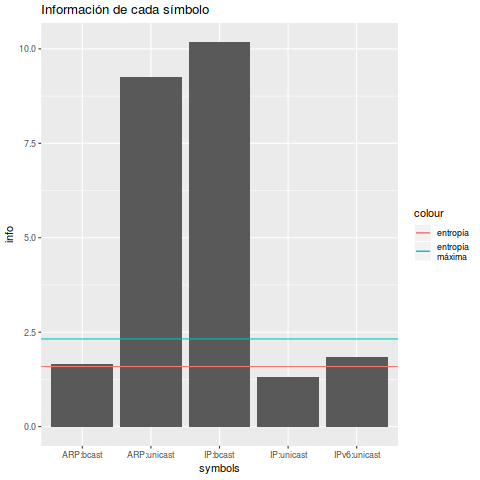
\includegraphics[scale=0.5]{s1/s1-casa-eric-nuevo-barras.png}
\end{center}

% ¿Se han encontrado símbolos distinguidos? ¿Les otorga algún significado?
% ¿La entropía de la fuente es máxima? ¿Bajo qué condiciones la entropía sería máxima? 
Se puede ver que la entropía de la fuente es menor a la entropía máxima. Esto
se debe a que no es uniforme la información de todos los símbolos: el símbolo
IP:broadcast contiene mucha más información que el IP:unicast. En términos más
palpables, esto quiere decir que es más predecible la red. Si uno tuviese que
adivinar cuál será el próximo paquete recibido, decir que será de tipo
IP:unicast tendría muchas chances de ser correcto.

Además, el símbolo IP:unicast es el único que posee información menor a la
entropía, haciéndolo mucho más común que los otros símbolos. De 45.143 paquetes
muestreados, 18.207 tuvieron este símbolo, haciendo que el 40,3\% de los paquetes
sean de este símbolo. Este es, definitivamente, un símbolo distinguido.

Como los paquetes de IP:unicast transportan en su mayoría datos de usuario,
que este símbolo sea distinguido indica que la red tiene buen goodput.


El porcentaje de paquetes para cada protocolo es de:
\begin{itemize}
	\item IP: 40,4\%
	\item IPv6: 27,7\%
	\item ARP: 31,9\%
\end{itemize}

El porcentaje de ARP en particular es muy parecido al del total de paquetes de
broadcast, lo que indica que tanto la cantidad de paquetes de broadcast de IP
como la de los paquetes de unicast de ARP son muy bajas.

% ¿Ha encontrado protocolos no esperados? ¿Puede describirlos?


% 2. Para S2: ¿La entropía de la fuente es máxima? ¿Qué sugiere esto acerca de la red? ¿Bajo qué con-
% diciones la entropía sería máxima? ¿Se pueden distinguir nodos? ¿Se les puede adjudicar alguna
% función específica? ¿Hay evidencia parcial que sugiera que algún nodo funciona de forma anómala
% y/o no esperada? ¿Existe una correspondencia entre lo que se conoce de la red y los nodos distinguidos
% detectados por la herramienta? ¿Ha encontrado paquetes ARP no esperados? ¿Cuál es su función?
\subsubsection{S2}

Utilizando el modelo que toma cada IP (ya sea fuente o destino) como
un símbolo distinto, vemos que en esta red tenemos un alfabeto
compuesto de 255 símbolos: los IPs del 192.168.0.1 a 192.168.0.254 y
la IP 0.0.0.0.

La entropía en el muestreo realizado en esta red dio un valor de
5,010991. Si comparamos la información de cada símbolo (estimando su
probabilidad de ocurrencia con la frecuencia empírica obtenida en la
muestra) con la entropía de la fuente calculada también con la
muestra, observamos que existe un único nodo distinguido, a saber el
nodo con el número 192.168.0.1, el cual tiene una frecuencia mucho
mayor y por ende una cantidad de información menor: es el único
símbolo que transmite una información menor a la entropía de la
fuente. Este hecho no es casual, ya que esa es la dirección IP correspondiente al
default gateway (de acuerdo al comando IP route corrido en la
computadora donde se realizó el muestreo), y probablemente sea, por lo
tanto, el router de la red.

En el grafo puede verse que el nodo correspondiente a este símbolo
tiene muchas aristas que lo
conectan con muchos de los otros nodos de la red, la gran mayoría de
los cuales solamente recibe paquetes del mismo, y de nadie más.

\begin{center}
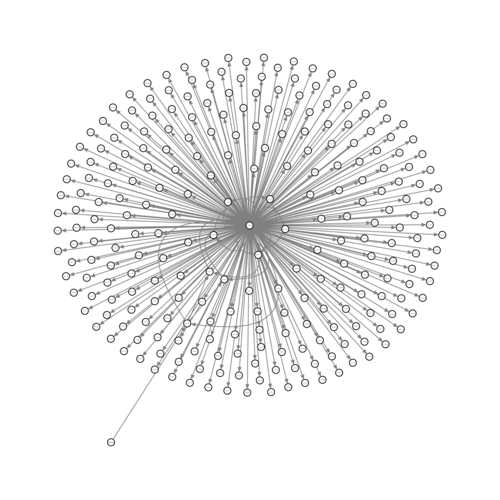
\includegraphics[scale=0.6]{../img/eric-lavarropas.png}
\end{center}

Al ver este grafo pensamos en considerar sólo aquellos nodos que son
tanto fuente como destino de algún paquete (es decir dejar
de considerar aquellos paquetes que el router 
envía a nodos que no envían ningún paquete).

\begin{center}
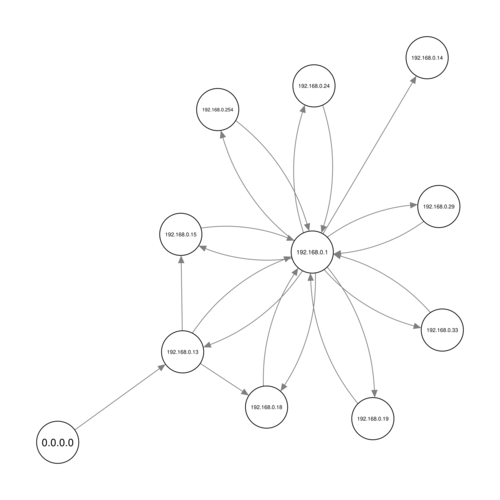
\includegraphics[scale=0.6]{../img/eric-flor.png}
\end{center}

En este grafo de menor tamaño puede verse el nodo 192.168.0.1 que
intercambia paquetes con todos los otros nodos (la mayoría de los
cuales sólo se comunican con él), y también el nodo 0.0.0.0.

La aparición del nodo 0.0.0.0 en la red es extraña, ya que no
puede pertenecer a un dispositivo. Investigando, descubrimos
que se utiliza como origen del paquete ARP WHO-HAS para saber si
ya existe un dispositivo con la dirección IP por la que se 
está preguntando. Lo mismo seguirá ocurriendo en las próximas
redes que analizaremos.

\subsection{Biblioteca Casa de la Lectura}
\subsubsection{S1}
% 1. Para S1: Mostrar la cantidad de infomación de cada símbolo comparando con la entropía de la fuente
% y la entropía máxima. Mostrar el porcentaje de tráfico broadcast sobre el tráfico total. Mostrar el
% porcentaje de aparición de cada protocolo encontrado.

% 1. Para S1: ¿Considera significativa la cantidad de tráfico broadcast sobre el tráfico total? 
El porcentaje de tráfico de broadcast en esta red es del 14,5\%. El tráfico unicast supera ampliamente
al broadcast en esta red en particular. Esto podría ocasionarse por el hecho de que los
usuarios de la biblioteca utilizan la red en conexiones largas, y por lo tanto los paquetes
de control de red son opacados por los de comunicación de datos. A continuación se muestra un
gráfico que nos ayudará a analizar mejor la muestra.

\begin{center}
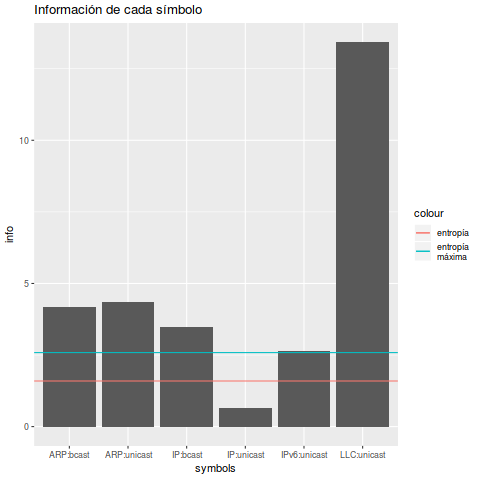
\includegraphics[scale=0.5]{s1/s1-biblio-s1-barras.png}
\end{center}


%¿Cuál es la función de cada uno de los protocolos encontrados? 
%¿Cuáles son de control y cuáles transportan datos de usuario? 

Se puede ver que el símbolo LLC:unicast es el que aporta mayor información.
Suponemos que son paquetes internos de la biblioteca, y que entonces son
superados en número por los paquetes enviados por los usuarios de la biblioteca.
También se puede ver que los IP:unicast son los que menos información brindan,
seguidos por los IPv6:unicast. Esto quiere decir que son los más enviados.
Estos son los paquetes que en su mayoría contienen datos de usuario,
a diferencia de los de ARP, que sirven para relacionar las direcciones IP con
las MAC de sus dueños; y los de IP:broadcast. Estos se utilizan para control de red.


% ¿Se han encontrado símbolos distinguidos? ¿Les otorga algún significado?

De nuevo, el único símbolo distinguido es el IP:unicast, que es el único cuya
información es menor a la entropía.

% ¿La entropía de la fuente es máxima? ¿Bajo qué condiciones la entropía sería máxima?
Podemos ver que la entropía en este caso tampoco es máxima, ya que hay mucha 
diferencia entre el símbolo de mayor información y el de menor información.

% ¿Ha encontrado protocolos no esperados? ¿Puede describirlos?
Podemos ver que algunos paquetes tienen protocolo LLC. Investigando, descubrimos
que es un protocolo de capa dos que permite multiplexar muchas fuentes de
información en una sola. En el caso particular de la biblioteca no
estamos seguros del uso que se les está dando.

El porcentaje de paquetes para cada protocolo es de:
\begin{itemize}
	\item IP: 73.4\%
	\item IPv6: 16.2\%
	\item ARP: 10.4\%
	\item LLC: 0.0\%
\end{itemize}

El porcentaje de paquetes de LLC es prácticamente cero, que se condice con lo
visto en el gráfico. Por otro lado, el porcentaje de paquetes IP supera con
creces a todos los demás.

\subsubsection{S2}

Utilizando el modelo S2 en esta muestra obtuvimos un
alfabeto de 178 símbolos. Estos son: la dirección IP 0.0.0.0, la 10.128.128.128,
la 10.5.47.7, 98 que empiezan con 10.92, 74 con 100.64 y por último
las 169.254.193.173 y 169.254.216.44. Las direcciones que empiezan con
10.96 pertenecen al rango 10.96.0.* a 10.96.15.*, con lo
que puede que pertenezcan a la red 10.92.0.0/20. Las direcciones que comienzan
con 100.64 están en el rango de 100.64.0.* a 100.64.31.*, por lo que
probablemente pertenezcan a la red 100.64.0.0/19.

La entropía encontrada en esta fuente de información es de 3.569424,
lo que da lugar a que existen tres nodos distinguidos (considerando a
aquellos cuya información es menor), a saber, los nodos
10.128.128.128, 100.64.22.24 y 100.64.0.1.

Dado que observando los números de direcciones supusimos que existían dos
subredes, quisimos observar los vínculos entre los distintos nodos
para ver el grafo subyacente. Es decir, graficamos el grafo que está
compuesto por aquellas aristas que conectan dos nodos de distinta
subred (además de que el grafo con todos los nodos y aristas obtenido
era demasiado grande para poder mirar en un gráfico), lo cual se ve a
continuación:

\begin{center}
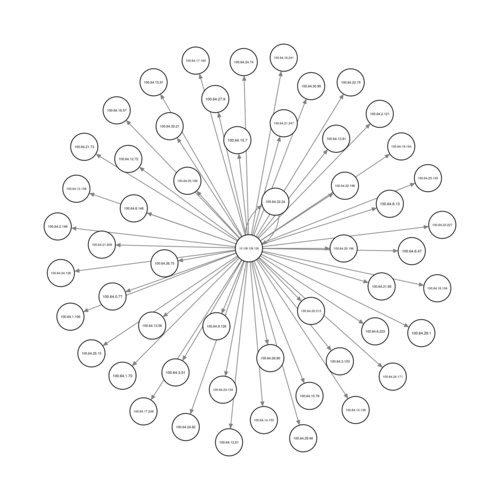
\includegraphics[scale=0.6]{../img/biblio-grafo-redesAB.png}
\end{center}

Puede verse en este grafo que los dos nodos distinguidos de mayor
ocurrencia están presentes: el 10.128.128.128 y el 100.64.22.24, los
cuales están conectados mediante dos aristas con orientaciones
diferentes (o sea cada uno envió algún paquete al otro). Por otra
parte, todos los demás nodos pertenecen a 100.64.0.0/19 y reciben
paquetes de 10.128.128.128 (son paquetes WHO-HAS).

Luego dibujamos otros dos grafos. El primero de ellos es el
resultante de sacar los nodos pertenecientes a 10.128 de la
red.

\begin{center}
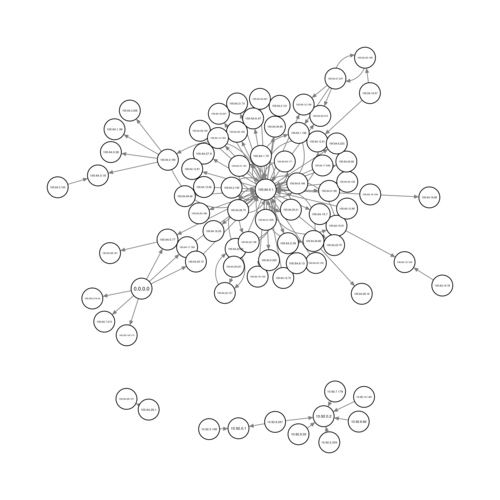
\includegraphics[scale=0.6]{../img/biblio-grafo-red-100-64.png}
\end{center}

En el centro se ve el nodo distinguido 100.64.0.1, que suponemos puede
ser un router dado que tiene aristas que los conectan con una gran
cantidad de otros nodos de la red. 

Por último, el grafo correspondiente a las aristas entre nodos no
pertenecientes a 10.128.

\begin{center}
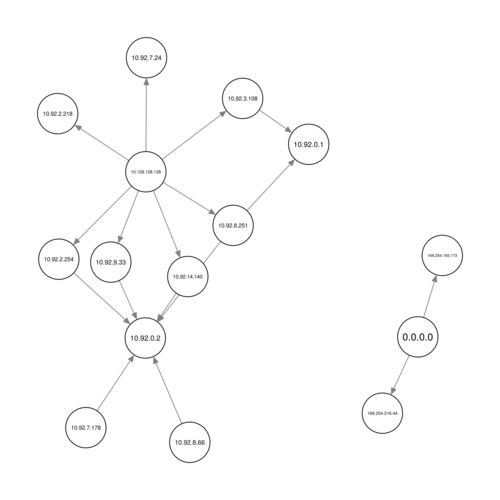
\includegraphics[scale=0.6]{../img/biblio-grafo-red-10-92.png}
\end{center}


\subsection{Red Pabellón 1}
\subsubsection{S1}
El porcentaje de tráfico de broadcast en esta red fue del 15,3\%. De nuevo, el
tráfico unicast lo supera ampliamente. Suponemos que ocurre lo mismo que en 
la muestra anterior: al tener más usuarios de la red enviando datos en 
sesiones largas, la cantidad de paquetes de control de red necesarios 
decrementa, que son en su mayoría de broadcast.
Esto podría derivar en un aumento del goodput, queriendo decir que cuantos 
más usuarios, mayor goodput.

A continuación se muestra el gráfico de barras correspondiente a esta red.

\begin{center}
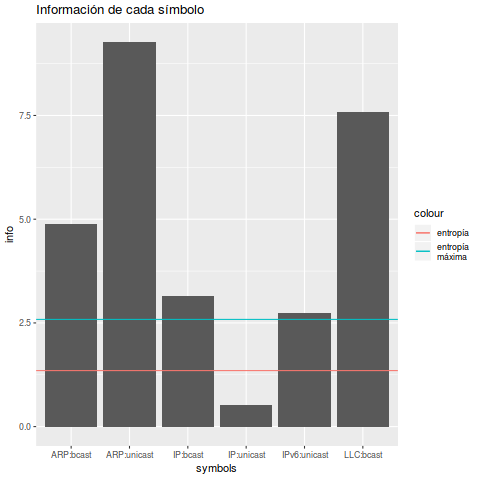
\includegraphics[scale=0.5]{s1/s1-exactas-wifi-barras.png}
\end{center}

%¿Cuál es la función de cada uno de los protocolos encontrados? 
%¿Cuáles son de control y cuáles transportan datos de usuario? 
Acá vemos más marcada la diferencia entre la información otorgada por el
símbolo IP:unicast y los demás. Además de indicar un mayor goodput, 
hace que la entropía baje en relación a la entropía máxima, ya que la
red es más predecible bajo este modelo. También está representado el
símbolo IPv6:unicast, lo que quiere decir que hay algunas comunicaciones
que se realizan con este protocolo más moderno.

% ¿Se han encontrado símbolos distinguidos? ¿Les otorga algún significado?

Una vez más podemos ver que el único símbolo distinguido es el IP:unicast.
% ¿La entropía de la fuente es máxima? ¿Bajo qué condiciones la entropía sería máxima?


% ¿Ha encontrado protocolos no esperados? ¿Puede describirlos?
En este caso se están mandando paquetes LLC:broadcast, a diferencia del caso
de la biblioteca, en el que se mandaban de LLC:unicast. Podemos inferir solamente
que el protocolo LLC es una forma genérica de enviar paquetes que cada administrador
de red puede adaptar a sus necesidades.


El porcentaje de paquetes para cada protocolo es de:
\begin{itemize}
\item IP: 81.0\%
\item IPv6: 14.9\%
\item ARP: 3.6\%
\item LLC: 0.5\%
\end{itemize}

En esta red parece haber más paquetes LLC que en el de la biblioteca, aunque la 
cantidad sigue siendo ínfima. El porcentaje de paquetes ARP también disminuyó,
que indica menos carga de red para paquetes de control. También el de paquetes
de IPv6, lo que quizá indica que el porcentaje de computadoras más modernas
es menor en la facultad que en la biblioteca. La disminución de la aparición
de los demás protocolos se ve reflejada en el incremento por parte del protocolo
IP.

\subsubsection{S2}
En esta red encontramos 209 símbolos, la mayoría de los cuales son 
direcciones IP
que comienzan con 10.2.200 a 10.2.203, y también hay direcciones
que comienzan con 169.254. De manera similar a la red de la biblioteca,
hicimos el grafo de los nodos con aristas que conectan ambas redes.

\begin{center}
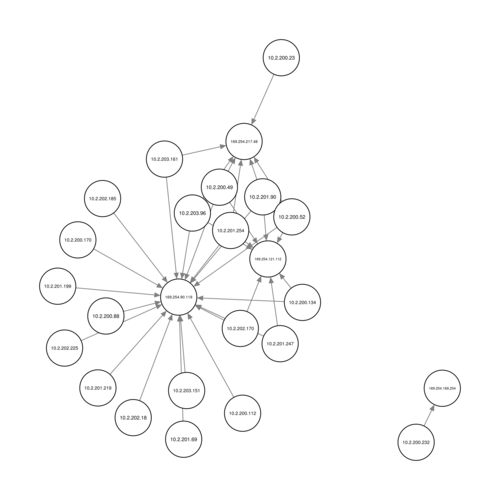
\includegraphics[scale=0.6]{../img/exactas-redesAB.png} 
\end{center}

Vemos de la red 169.254 que el nodo 169.254.119 recibe muchos
paquetes. Cabe destacar que si bien la información de dicha dirección
resulta mayor al valor de entropía de la red (es decir que no es tan
frecuente), es el de mayor frecuencia entre las direcciones 169.254.

En el grafo en el cual sacamos los nodos de 10.2, podemos ver que
en su mayoría se trata de paquetes con destino 0.0.0.0.

\begin{center}
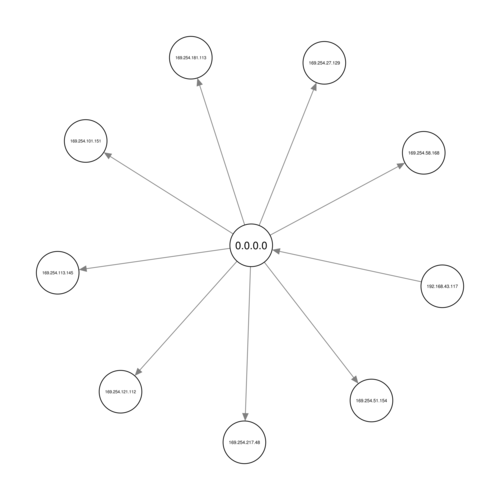
\includegraphics[scale=0.5]{../img/exactas-sin10-2.png}
\end{center}

Por último, el grafo de la red Pabellón 1 al que le sacamos los nodos
169.254 está compuesto de una gran cantidad de nodos, destacándose
la posición en el grafo del nodo 10.2.203.254, que es el de mayor
frecuencia.

\begin{center}
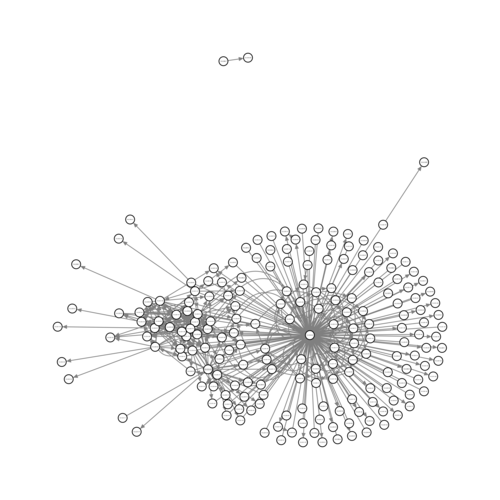
\includegraphics{../img/exactas-sin169.png}
\end{center}
